\chapter{Design Features and Implementation} % Main chapter title
\label{chap:Chapter4}  % For referencing the chapter elsewhere, use \ref{Chapter4}

\epigraph{”Our goals can only be reached through a vehicle of a plan, in which we must fervently believe, and upon which we must vigorously act. There is no other route to success." }{\textit{Pablo Picasso}}

Στο παρόν κεφάλαιο περιγράφεται η διαδικασία σχεδιασμού και υλοποίησης του \Abbr{MoCap} με χρήση drone swarm συστήματος, που συσχετίζεται η παρούσα διπλωματική. 

Μία high-level προσέγγιση, θα μπορούσε να διαχωρίζει το σύστημα σε τρία διακριτά
υποσυστήματα. Αρχικά το optical, του οποίου αρμοδιότητα είναι το detection, το tra\-cking, καθώς και η εκτίμηση
του range ή γωνίας του αντικειμένου από την camera. Δεύτερο, η λήψη των πληροφοριών από τους αισθητήρες ώστε να προσεγγιστεί η θέση του ίδιου
του drone. Τέλος, ο συνδυασμός των δύο παραπάνω μερών και η χρήση κατάλληλης localization τεχνικής για να βρεθεί η θέση του αντικειμένου
στο \Abbr{3D} χώρο.

%----------------------------------------------------------------------
\section{Equipment and Tools Used} \label{sec:design-tools}
Αρχικά θα αναφερθούν συνοπτικά η αρχιτεκτονική στην οποία έγινε επιλογή να επιλυθεί το πρόβλημα,
όπως επίσης και τα εξαρτήματα/αισθητήρια όργανα καθώς και τα λογισμικά τα οποία χρησιμοποιήθηκαν στην παρούσα διπλωματική. 

\subsection{Embedded Linux System}
Δύο πολύ δημοφιλείς επιλογές στον χώρο των ενσωματωμένων συστημάτων - ως κεντρικές μονάδες επεξεργασίας - είναι οι πλακέτες Raspberry Pi που κατασκευάζονται από την Raspberry Pi Foundation σε συνεργασία με την Broadcom, καθώς και οι πλακέτες Jetson της Nvidia. Στο \Fig{embedded-linux-systems} ως παράδειγμα παρουσιάζονται ενδεικτικά μία εκδοχή από την κάθε οικογένεια, ενώ στα \Tabl{raspberry-pi-specs} και \Tabl{jetson-nano-specs} τα τεχνικά χαρακτηριστικά της εκάστοτε πλακέτας ως αρχικό σημείο αναφοράς. 

\begin{figure} [H]
	\centering
	% -----------------
    \begin{minipage}{.5\textwidth}
      \centering
      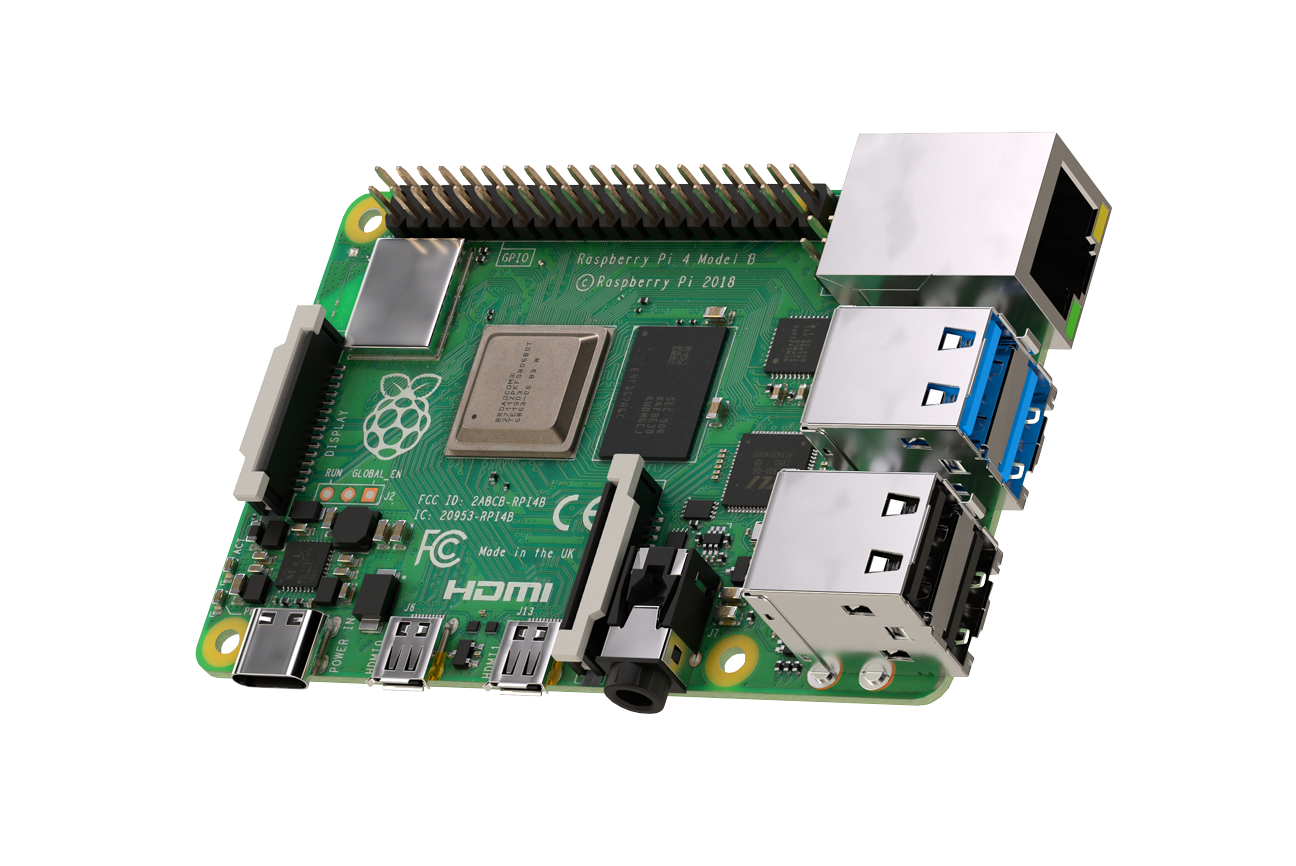
\includegraphics[width=\linewidth]{Images/Design-Implementation/raspberry-pi-4.png}\\
      {(a) Raspberry Pi 4 \URI{https://www.hellasdigital.gr/go-create/raspberry-and-accessories-el/raspberry-pi/raspberry-pi-4-4gb-ram/}}
    \end{minipage}%
    % -----------------
    \begin{minipage}{.5\textwidth}
      \centering
      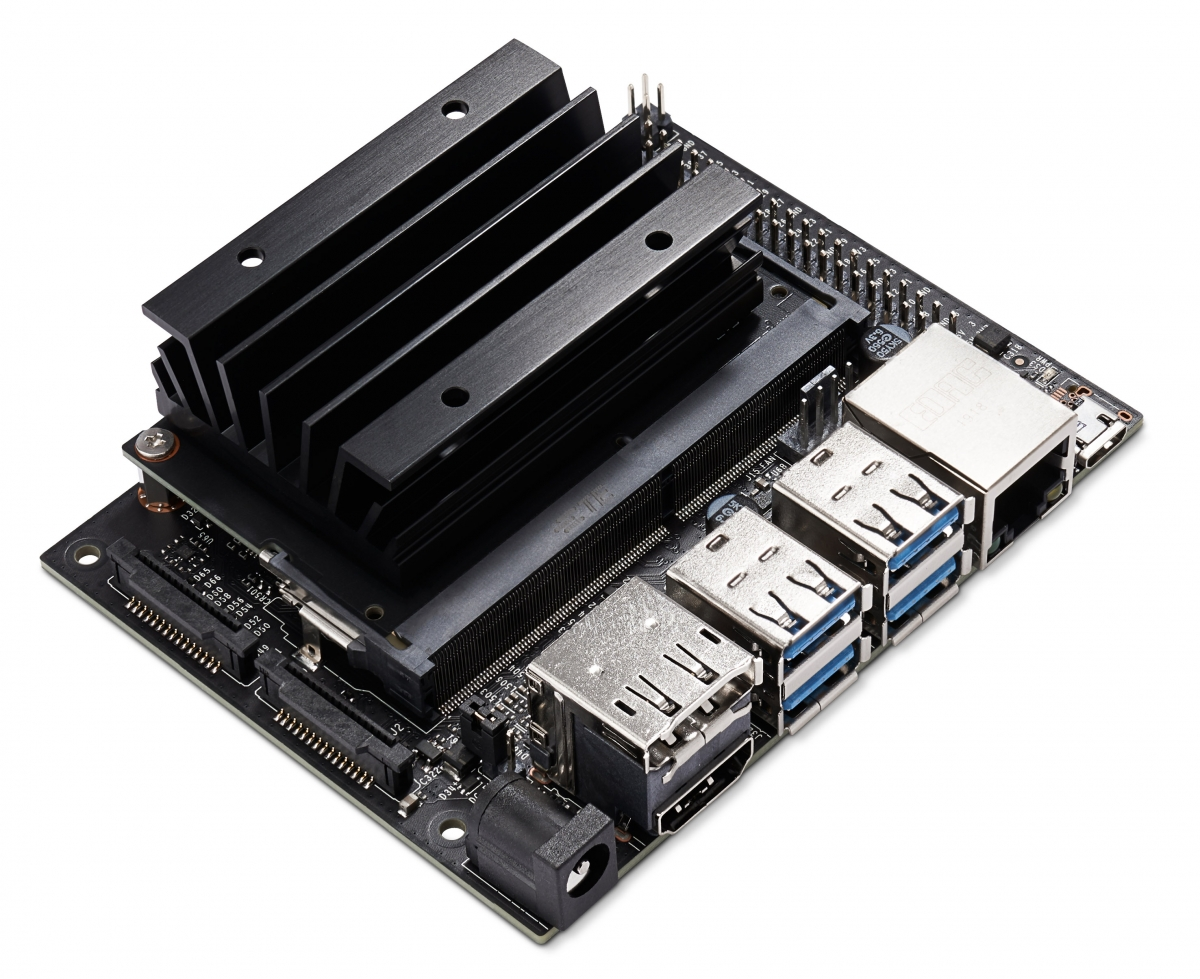
\includegraphics[width=.9\linewidth]{Images/Design-Implementation/jetson-nano.jpeg}\\
      {(b) Jetson Nano \URI{https://www.hellasdigital.gr/computers/accessories/nvidia-jetson-nano-developer-kit/}}
	\end{minipage}
	% -----------------
    \hfill \break
    \decoRule
    \CaptionBasedwithURL{Possible Embedded Linux Systems} 
    \label{fig:embedded-linux-systems}
\end{figure}

Και οι δύο επιλογές αποτελούνται από έναν ARM αρχιτεκτονικής Central Processing Unit (\Abbr{CPU}), ενώ στις Jetson βρίσκεται επιπρόσθετα και ένα Graphics Processing Unit (\Abbr{GPU}) που μπορεί να χρησιμοποιηθεί σε ενσωματωμένα με μεγάλες ανάγκες επεξεργασίας (όπως αυτά που σχετίζονται με εικόνα/βίντεο).

\begin{table}[H]
    \caption[]{Raspberry Pi 4 Model B Specifications}
    \label{tab:raspberry-pi-specs}
    \centering
    \resizebox{.63\textwidth}{!}{
        \begin{tabular}{ll}
            \hline
            \textbf{Feature} & \textbf{Value}  \\
            \hline
                Processor & \Centerstack{Broadcom BCM2711, Quad core Cortex-A72 \\(ARM v8) 64-bit SoC @ 1.5GHz }\\
                Memory & 8GB LPDDR4-3200 SDRAM \\
                Storage & External Micro-SD \\  
                Power & 5V DC (maximum 3A), 5-15Watt \\
                Cost & $\sim$100 €\\
                Weight & 46 grams (without case), 99 grams (with case) \\
                Peripherals & GPIO, I2C, SPI, UART \\
                \hline
        \end{tabular}
    }
  \end{table}

  Στην συγκεκριμένη διπλωματική επιλέχθηκε η ανάπτυξη του συστήματος να γίνει σε Raspberry Pi 4 boards - λόγω του ελάχιστα μικρότερου κόστους καθώς και μάζας τους - έχοντας μελλοντικά την επιλογή για migration ενός ή περισσότερων κόμβων του συστήματος σε Jetson boards, αν κριθεί αυτή η ανάγκη, για λόγους σχετικούς με την ταχύτερη επεξεργασία των δεδομένων.

  \begin{table}[H]
        \caption[]{Jetson Nano Developer Kit Specifications}
        \label{tab:jetson-nano-specs}
        \centering
        \resizebox{.63\textwidth}{!}{
            \begin{tabular}{ll}
                \hline
                \textbf{Feature} & \textbf{Value}  \\
                \hline
                    CPU & Quad-core ARM Cortex-A57 MPCore processor\\
                    GPU & \Centerstack{NVIDIA Maxwell architecture with 128 NVIDIA\\ CUDA® cores} \\
                    Memory & 4 GB 64-bit LPDDR4; 25.6 gigabytes/second \\
                    Storage & External Micro-SD \\  
                    Power & 5V DC, 5-10Watt \\
                    Cost & $\sim$120€\\
                    Weight & 250 grams (without case)\\
                    Peripherals & GPIO, I2C, I2S, SPI, UART \\
                    \hline
            \end{tabular}
        }
      \end{table}

% -----------------

\subsection{ROS} \label{sec:ROS}
Συνδετικός κρίκος των υποσυστημάτων είναι το open-source middleware Robot Operation System (\Abbr{ROS}) \cite{ros} το οποίο 
πε\-ρι\-λα\-μβά\-νει ένα εκτενές σύνολο εργαλείων, βιβλιοθηκών και συ\-μβά\-σεων. Τα πακέτα του οποίου χρησιμοποιούνται για την
λήψη και φιλτράρισμα από τους αισθητήρες των πληροφοριών, επικοινωνία μεταξύ των drone όπως τέλος και 
όποια τρι\-σδιά\-στα\-τη απεικόνιση χρειάζεται.

Μεγάλο πλεονέκτημα του \Abbr{ROS} είναι η ύπαρξη των packages. Τα packages είναι δια\-κρι\-τά αυτόνομα κομμάτια κώδικα τα οποία περικλείουν μία συχνά επαναλαμβανόμενη λογική, συνεπώς μπορούν να χρησιμοποιηθούν αυτούσια - με πολύ εύκολο τρόπο - σε διαφορετικές εφαρμογές χωρίς να υπάρχει η ανάγκη να κάνουμε \textit{reinvent the wheel} κάθε φορά, πετυχαίνοντας με αυτό τον τρόπο το rapid prototyping and testing ενός συστήματος καθώς και την αποφυγή δημιουργίας boilerplate κώδικα δίνοντας έμφαση περισσότερο στο main logic του εκάστοτε συστήματος. 

Το \Abbr{ROS} στην πραγματικότητα είναι ένα meta-operating system, με αποτέλεσμα να χρειάζεται να τρέχει σε ένα πρωτεύον Operating System (\Abbr{OS}), συγκεκριμένα μέχρι αυτήν την στιγμή απαιτεί την χρήση Ubuntu Linux. 

Πηγές οι οποίες χρησιμοποιήθηκαν για την εκμάθηση του \Abbr{ROS} ήταν

% -----------------
\subsection{Operation System}
Από την στιγμή που επιλέχθηκε να γίνει χρήση του \Abbr{ROS} - που όπως αναφέρθηκε στο \Sect{ROS} απαιτεί την χρήση Ubuntu Linux - έγινε εγκατάσταση στο Raspberry Pi η ειδικά σχεδιασμένη για το αυτό έκδοση Ubuntu Linux 20.04.2 64bit version για ΑRM \cite{ubuntu-raspberry} αρχιτεκτονική. Ουσιαστικά όλες οι λειτουργίες της εφαρμογής θα χρησιμοποιούν το Embedded General Purpose Operating System προκειμένου να λειτουργήσουν, το οποίο σημαίνει ότι αυτό θα είναι κυρίως υπεύθυνο για το scheduling, file-system abstraction, networking, etc. 

% -----------------
\subsection{OpenCV}
Για το οπτικό σκέλος χρησιμοποιήθηκε η ανοιχτού κώδικα βιβλιοθήκη OpenCV \cite{opencv}, η οποία αποτελεί την δημοφιλέστερη επιλογή για real-time Computer Vision related εφαρμογές. Ξεκίνησε η ανάπτυξη της στα εργαστήρια της Intel και έχει ήδη διάρκεια ζωής λίγο περισσότερο από δύο δεκαετίες. Για τις ανάγκες στης συγκεκριμένης εργασίας χρησιμοποιήθηκε η έκδοση της 4.2.0. 

% -----------------
\subsection{Camera}
Σχετικά με την κάμερα, ήταν ανάγκη - όντας πρώτη γενιά του συστήματος -  να επιλεχθεί μία low-cost 1080p camera η οποία θα παρέχει δυνατότητα επιλογής χαμηλότερου resolution για λόγους δοκιμών. Στο πρωτότυπο σύστημα τελικά γίνεται χρήση μία 1080p web cameras της Creative \cite{creative-camera} - \Fig{creative-camera} - με δυνατότητες λήξης βίντεο στα 30fps, η οποία συνδέεται μέσω USB στο Raspberry Pi.

% Image
\FigCaptLabelBasedURL{Images/Design-Implementation/creative-web-cam.jpeg}%
{Camera used for ball detection and tracking}%
{creative-camera}%
<0.35>%
(https://en.creative.com/p/peripherals/creative-live-cam-sync-1080p)


% -----------------
\subsection{GPS} \label{sec:GPS}
Παρόλο που - όπως αναφέρθηκε στο \Chap{thesis-approach} - στο συγκεκριμένο σύστημα μας ενδιαφέρει το relative positioning και όχι το absolute, σκεπτόμενοι ότι στην πραγματικότητα το σύστημα σχεδιάζεται με γνώμονα το να λειτουργεί σε outdoor scenarios\udot ένας άμεσος τρόπος προσδιορισμού της θέσης του κάθε drone είναι με χρήση κάποιου εμπορικού αισθητήρα \Abbr{GPS}. Στην συνέχεια και αφού έχει αποκτηθεί πληροφορία απόλυτης θέσης για το κάθε drone μπορεί - θεωρώντας ένα από αυτά ως αρχή των αξόνων - να γίνει translate των απόλυτων συντεταγμένων ώστε να κρατηθεί μόνο πληροφορία σχετικά με την χωρική τοπολογία του δικτύου.

Συγκεκριμένα, χρησιμοποιείται το \Abbr{GPS} για commercial χρήση ΒΝ-220 \cite{bn-220-gps} - \Fig{bn-220-gps} - το οποίο υπόσχεται εμβέλειας ακρίβειας της τάξης των δύο μέτρων. Πρακτικά, παρόλο που για ένα \Abbr{MoCap} σύστημα αυτή η τιμή είναι απαγορευτική, χρησιμοποιείται στα πρώτα versions, καθαρά αναφορικά με την εξικοίωση του τρόπου επικοινωνίας \Abbr{ROS} - \Abbr{GPS}. Σε επόμενα revisions σκοπός είναι η αντικατάσταση του με \Abbr{RTK}-\Abbr{GPS} που συχνά μπορεί να φέρουν drone για αυτήν την χρήση ώστε να φτάσει η συνολική ακρίβεια εκτίμησης της απόλυτης θέσης στα μερικά εκατοστά. 

Το συγκεκριμένο \Abbr{GPS} συνδέεται με το Raspberry Pi μέσω Universal Asynchronous Receiver-Transmitter (\Abbr{UART}) \cite{uart-protocol} σύνδεσης και χρησιμοποιεί NMEA-0183 \cite{NMEA-0183-packets} πακέτα για την επικοινωνία. 

\FigCaptLabelBasedURL{Images/Design-Implementation/bn220.png}%
{GPS module used to estimate position}%
{bn-220-gps}%
<0.35>%
(https://www.google.com/imgres?imgurl=https\%3A\%2F\%2Fimages.jdmagicbox.com\%2Fquickquotes\%2Fimages_main\%2Fb07wwx5jvp-electroprime-bn-220-3-0v-5-0v-ttl-level-gnss-module-gps-glonass-dual-gps-module-antenna-v4b2-181504802-qn443.jpg&imgrefurl=https\%3A\%2F\%2Fwww.justdial.com\%2FELECTROPRIME-BN-220-3-0V-5-0V-TTL-Level-Gnss-Module-GPS-Glonass-Dual-GPS-Module-Antenna-V4B2\%2Fpid-181504802&tbnid=YJcAk2WsHSEZiM&vet=10CF8QMyiOAWoXChMI2M3PyrCA8wIVAAAAAB0AAAAAEAk..i&docid=xDxMDFHprlF2iM&w=500&h=500&itg=1&q=bn-220\%20image&hl=el&client=ubuntu&ved=0CF8QMyiOAWoXChMI2M3PyrCA8wIVAAAAAB0AAAAAEAk)

% -----------------
\subsection{IMU}\label{sec:imu}
Ήδη από το \Sect{Chapter1-1-2} έχει γίνει αναφορά για την σημαντικότητα των \Abbr{IMU}, καθώς αποτελούν τα κύρια αισθητήρια όργανα καθορισμού σε πολλαπλούς άξονες της σχετικής θέσης/κίνησης του drone. Επιλέχθηκε να χρησιμοποιηθεί το \Abbr{IMU} \cite{adafruit-10dof-imu} της Adafruit - \Fig{adafruit-10DoF-imu} - το οποίο παρέχει 10-\Abbr{DoF}, με onboard αισθητήρες ένα τριών αξόνων accelerometer, τριών αξόνων gyroscope, τριών αξόνων magnetometer (compass), ένα barometric pressure/altitude αισθητήρα και δυνατότητα υ\-πο\-λο\-γι\-σμού της θερμοκρασίας.

Θετικό του συγκεκριμένου module είναι ότι όλοι οι παραπάνω αισθητήρες είναι συ\-νδε\-δε\-μέ\-νοι σε ένα κοινό Inter-Integrated Circuit (\Abbr{I2C}) \cite{I2C-protocol} bus, μέσω του οποίου μπορεί πολύ εύκολα να γίνει η διασύνδεση με την επεξεργαστική μονάδα που επιθυμούμε και να πραγματοποιηθεί επικοινωνία. 

% Image
\FigCaptLabelBasedURL{Images/Design-Implementation/10DoF-Adafruit-IMU.jpeg}%
{Adafruit 10 DoF IMU}%
{adafruit-10DoF-imu}%
<0.35>%
% ()

% -----------------
\subsection{Breakout Board}
Για να λειτουργήσουν τα παραπάνω υποσυστήματα, χρειαζόταν να πραγματοποιηθούν οι κατάλληλες φυσικές διασυνδέσεις. Η απλούστερη εκδοχή θα ήταν να γίνει αυτό με χρήση breadboard, πράγμα όμως που θα πρόσθετε όγκο και βάρος στο τελικό σύστημα, οι οποίοι σε περίπτωση δοκιμών πάνω σε πραγματικά drone να είναι απαγορευτικοί παράγοντες. Συνεπώς, προκειμένου να μπορεί με ευκολία να γίνει η ανάπτυξη του συστήματος, σχεδιάστηκε (στο cad εργαλείο KiCad \cite{KiCad}) και κατασκευάστηκε ένα custom breakout board\footnote{Είναι διαθέσιμο ως open hardware project στο \cite{raspberry-pi-fan-breadkout}} όπως φαίνεται στο \Fig{raspberry-pi-breakout}. Αυτό παρέχει εύκολη πρόσβαση στα GPIO του Raspberry, έξτρα pins για τροφοδοσία στα 5 και 3.3 Volt, pins για τοποθέτηση αισθητήρων - όπως του \Abbr{IMU} - καθώς και mounting holes στα οποία μπορεί να τοποθετηθεί 40x40mm fan για την ψύξη του συστήματος. 

% Image
\FigCaptLabelBasedURL{Images/Design-Implementation/Rpi-breakout.png}%
{Raspberry Pi breakout}%
{raspberry-pi-breakout}%
<0.50>


% -----------------
\subsection{System Overview}
Η ολοκληρωμένη μορφή του πρωτότυπου συστήματος παρουσιάζεται στο \Fig{thesis-system}, ενώ στο \Tabl{thesis-system-bom} μπορούν να βρεθούν συνολικά τα εξαρτήματα που χρησιμοποιήθηκαν μαζί με την κοστολόγηση τους. 

Το σύστημα ζυγίζει $\sim$ 250gr, μία αρχική εκτίμηση κατανάλωσης είναι τα 15 watt και οι εξωτερικές διαστάσεις του είναι 17x7.5x10.5cm.

% Image
\FigCaptLabelBasedURL{Images/Design-Implementation/thesis-system.jpg}
{System designed}%
{thesis-system}%
<0.65>

\begin{table}[H]
    \caption[]{Bill of Materials}
    \label{tab:thesis-system-bom}
    \centering
    \resizebox{0.55\textwidth}{!}{
        \begin{tabular}{ll}
            \hline
            \textbf{Component} & \textbf{Cost}  \\
            \hline
                Raspberry Pi 4 Model B 8GB & \Centerstack{$\sim$ 100 €}\\
                Creative live cam sync 1080p \cite{creative-camera} & \Centerstack{$\sim$ 44 €}\\
                Adafruit 10 DoF IMU \cite{adafruit-10dof-imu} & \Centerstack{$\sim$ 30 €}\\
                BN-220 GPS Module \cite{bn-220-gps} & \Centerstack{$\sim$ 15 €}\\
                Breakout Board with fan \cite{raspberry-pi-fan-breadkout} & \Centerstack{$\sim$ 8 €}\\
                \hline
        \end{tabular}
    }
  \end{table}


% ------------------------------------------------------------------------------------------------------
\section{Environment}
Έχοντας ήδη αναφερθεί σε όλα τα υποσυστήματα που χρησιμοποιούνται, σε αυτό το section θα δοθεί ο τρόπος με τον οποίο διαμορφώθηκαν/προγραμματίστηκαν ώστε να λειτουργούν μεταξύ τους.

\subsection{Operation System} 
Στο \cite{ubuntu-raspi-intall} βρίσκονται αναλυτικές οδηγίες εγκατάστασης του Ubuntu στο Ra\-spbe\-rry Pi, ανάλογα με το λειτουργικό που ήδη χρησιμοποιούμε. Στην συγκεκριμένη περίπτωση - επειδή η εγκατάσταση έγινε από διανομή Linux - αφού έγινε λήψη του pre-made image του Ubuntu, βρέθηκε το path της SD card στον υπολογιστή, στην οποία έγινε umount, και στην συνέχεια χρησιμοποιήθηκε η εντολή dd για την δημιουργία του bootable μέσου, με τον εξής τρόπο.

\begin{lstlisting}[language=sh, escapechar=@, caption={Create bootable SD from Linux},label=create-bootable-sd-terminal]
    @\color{dkgreen}{\$}@ sudo dd bs=4M @if@=PATH_TO_YOUR_IMAGE_FILE of=PATH_TO_YOUR_SD_CARD status=progress
\end{lstlisting}

Μόλις ολοκληρωθεί η παραπάνω διαδικασία, το λειτουργικό σύστημα είναι έτοιμο προς χρήση. Αφού έγινε update του συστήματος, έγιναν οι εξής παραμετροποιήσεις. Αρχικά απενεργοποιήθηκε το Graphical User Interface κατά την διάρκεια του boot, επίσης απενεργοποιήθηκε το auto-suspend μετά από χρονικό διάστημα μη χρήσης, και τέλος εγκαταστάθηκαν οι εφαρμογές/πακέτα/βιβλιοθήκες - όπως το \Abbr{ROS} - που είναι απαραίτητα για την υλοποίηση του συστήματος. 

Σε αυτό το σημείο να αναφερθεί ότι χρησιμοποιήθηκε η έκδοση noetic του \Abbr{ROS}.

% ROS Packages(\TODO{update them}):
% \begin{itemize}
%   \addtolength{\itemindent}{0.3cm}
%   \item tf2\_ros
%   \item robot\_localization
%   \item usb\_cam
%   \item nmea\_navsat\_driver
% \end{itemize}

% -------------------------
\subsection{Sensors' Communication} 
Στο σημείο που ολοκληρώθηκαν οι παραπάνω απαραίτητες ενέργειες, υπήρχε  πλέον ένα λειτουργικό περιβάλλον, οπότε και ξεκίνησε η διαδικασία πραγματοποίησης ε\-πι\-τυ\-χη\-μέ\-νης επικοινωνίας με το κάθε υποσύστημα.

%---------------------------
\subsubsection{Serial Communication}
Πρώτα θα αναφερθεί η επικοινωνία με το \Abbr{GPS} η οποία όπως αναφέρθηκε στο \Sect{GPS} γίνεται μέσω \Abbr{UART}. Η σειριακή port του Raspberry μπορεί να γίνει access μέσω του αρχείου \textit{/dev/ttyS0}. Ενώ, για να μπορεί να προσπελαστεί από τον χρήστη χρειάστηκε να γίνουν τα βήματα \cite{serial-fix} που υπάρχουν στο \List{fix-serial-communication}.

% \begin{enumerate}
%     \item Να προστεθεί η γραμμή `enable\_uart=1' στο αρχείο \textit{/boot/config.txt}
%     \item Να αφαιρεθεί το `console=serial0,115200' από το αρχείο \textit{/boot/firmware/cmdline.txt}
%     \item 
% \end{enumerate}

\begin{lstlisting}[language=bash, escapechar=?, caption={Fix serial communication},label=list:fix-serial-communication]
    # 1. Add `enable_uart=1' to /boot/config.txt file
    sudo bash -c '?echo "enable\_uart=1"? >> /boot/config.txt'

    # 2. Remove `console=serial0,115200' from /boot/firmware/cmdline.txt
    sudo ?sed -e "s/console=serial0,115200//g"? -i /boot/firmware/cmdline.txt

    # 3. Disable serial console service
    sudo systemctl stop serial-getty@ttyS0.service
    sudo systemctl disable serial-getty@ttyS0.service

    # 4. Give privileges to user
    sudo adduser $USER tty
    sudo adduser $USER dialout
    sudo chmod g+r /dev/ttyS0
\end{lstlisting}

Μετά την εκτέλεση τους, συνδέοντας κατάλληλα τα RX - TX του \Abbr{GPS} στο Ra\-spbe\-rry, είναι εφικτό κάνοντας run την εντολή `\textbf{cat /dev/ttyS0}' να έχουμε πρόσβαση στα πακέτα NMEA που στέλνει το \Abbr{GPS}, που έχουν μορφή παρόμοια με το \List{serial-output}.

\begin{lstlisting}[language=bash, escapechar=@, caption={Serial Output, NMEA packets example},label=list:serial-output]
    ...
    $GNGSA,A,1,,,,,,,,,,,,,99.99,99.99,99.99*2E
    $GPGSV,1,1,01,31,,,13*78
    $GLGSV,1,1,00*65
    $GNGLL,,,,,180928.00,V,N*5E
    ...
\end{lstlisting}

Προκειμένου το \Abbr{ROS} να χρησιμοποιεί το \Abbr{GPS}, χρειάστηκε να εγκατασταθεί το πακέτο \textbf{nmea\_navsat\_driver} \cite{nmea-navsat-driver} και παράδειγμα χρήσης αυτού με το \Abbr{ROS} υπάρχει στο \List{gps-ros-sample-usage}.  

\begin{lstlisting}[language=bash, escapechar=@, caption={GPS - ROS sample usage},label=list:gps-ros-sample-usage]
    rosrun nmea_navsat_driver nmea_serial_driver _port:=/dev/ttyS0 _baud:=9600 
\end{lstlisting}

Σημαντικό είναι να αναφερθεί ότι η σειριακή θύρα χρησιμοποιείται για Debug λόγους κατά το boot
του Raspberry Pi, συνεπώς το \Abbr{GPS} πρέπει να μην είναι συνδεδεμένο αρχικά και μόνο αφού ολοκληρωθεί το boot να συνδεθεί στο σύστημα.

%---------------------------
\subsubsection{I2C communication}
Σε αντίθεση με την σειριακή επικοινωνία, το \Abbr{IMU} module χρησιμοποιεί το \Abbr{I2C} πρωτόκολλο (βλ. \Sect{imu}).
Για να μπορέσουμε να χρησιμοποιήσουμε το \Abbr{I2C} στο Raspberry, χρειάστηκε να εκτελεστούν οι εντολές που υπάρχουν στο \List{fix-I2C-communication}.

\begin{lstlisting}[language=bash, escapechar=@, caption={Fix I2C communication},label=list:fix-I2C-communication]
    # 1. Install cpp needed library
    sudo apt-get install -y libi2c-dev 

    # 2. Give privileges to user
    sudo adduser $USER i2c
    sudo chmod g+r /dev/i2c-1
\end{lstlisting}

Στην συνέχεια μπορούν να γίνουν οι κατάλληλες συνδέσεις και εκτελώντας την εντολή `\textbf{i2cdetect -y 1}' να εμφανιστούν
οι διευθύνσεις όλων των αισθητήρων που είναι συνδεδεμένες στο \Abbr{I2C} bus, παράδειγμα του output από την εντολή υπάρχει στο \List{I2C-output}.

\begin{lstlisting}[language=bash, escapechar=@, caption={I2C addressed output example},label=list:I2C-output]
    0  1  2  3  4  5  6  7  8  9  a  b  c  d  e  f
    00:          -- -- -- -- -- -- -- -- -- -- -- -- -- 
    10: -- -- -- -- -- -- -- -- -- 19 -- -- -- -- 1e -- 
    20: -- -- -- -- -- -- -- -- -- -- -- -- -- -- -- -- 
    30: -- -- -- -- -- -- -- -- -- -- -- -- -- -- -- -- 
    40: -- -- -- -- -- -- -- -- -- -- -- -- -- -- -- -- 
    50: -- -- -- -- -- -- -- -- -- -- -- -- -- -- -- -- 
    60: -- -- -- -- -- -- -- -- -- 69 -- -- -- -- -- -- 
    70: -- -- -- -- -- -- -- 77       
\end{lstlisting}

Η επίσημη βιβλιοθήκη της Adafruit για το module 
\TODO{about ROS package}

%----------------------------------------------------------------------

Notes
\section{Camera} \label{sec:design-implementation-camera}
image as a function from  
2d projection of 3d points
losing 3rd dimension

lens are not perfect
- geometric lens distortion
- ακόμα και chromatic aberration
- vignetting

\begin{gather}
	\phi = \taninv{\left( \frac{d/2}{f} \right)}
\end{gather}


Perspective Projection equation:
\begin{gather}
	(X, Y, Z) \rightarrow (-d \frac{X}{Z}, -d \frac{Y}{Z}, -d)
\end{gather}

"we get the projection by throwing out the last coordinate"
\begin{gather}
	(x', y') \rightarrow (-d \frac{X}{Z}, -d \frac{Y}{Z})
\end{gather}

"Obvious application of this dividing by z, is that distant objects are smaller in the image"

"Zero is the center of the image"

Homogeneous Coordinates or homogeneus component of the vector

$\frac{X}{Z}$ and $\frac{Y}{Z}$ is not a linear transformation because Z is not constant so, we add one more coordinate $(x/w,y/w) \Leftrightarrow \begin{bmatrix} x \\ y \\ w \end{bmatrix} $ for (2d) coordinates, Homogeneous image
and $(x/w,y/w,z/w) \Leftrightarrow \begin{bmatrix} x \\ y \\ z \\w \end{bmatrix} $ for (3d) coordinates, Homogeneous scene.

this makes homogeneout coordinates invariant under scale

so now perspective projection is like that

use homogeneous coordinates to do matrix operations without the fear on non linearity until the very end
\begin{gather}
	\begin{bmatrix} 
        1 & 0 & 0 & 0 \\ 
        0 & 1 & 0 & 0 \\ 
        0 & 0 & 1/f & 0 \\
    \end{bmatrix} 
    \begin{bmatrix} x \\ y \\ z \\ 1 \end{bmatrix}
    =
    \begin{bmatrix} x \\ y \\ z/f \end{bmatrix}
    \Rightarrow
    \left( f\frac{x}{z}, f\frac{y}{z} \right)
    \Rightarrow
    (u,v)
\end{gather}

projection matrix is $\begin{bmatrix} 1 & 0 & 0 & 0 \\ 0 & 1 & 0 & 0 \\ 0 & 0 & 1/f & 0 \\\end{bmatrix}$

u, v points in the image of some point x,y,z in the world

points go to points
lines go to lines
polygons go to polygons

\begin{table}[H]
    \caption[Three camera projections]{Three camera projections}
	\label{tab:three-camera-projections}
	\centering
	\resizebox{.8\textwidth}{!}{
		\begin{tabular}{lllll}
			\toprule
			 & & \Centerstack{3D point} & & 2D image\\
			\midrule
            $\imath$. & Perspective: & $(x,y,z)$ & $\rightarrow$ & $\left(\frac{fx}{z}, \frac{fy}{z}\right)$ \\ 
            $\imath\imath$. & Weak perspective & $(x,y,z)$ & $\rightarrow$ & $\left(\frac{fx}{z_0}, \frac{fy}{z_0}\right)$ \\ 
            $\imath\imath\imath$. & Orthographic & $(x,y,z)$ & $\rightarrow$ & $(x,y)$ \\ 
			\bottomrule
		\end{tabular}
	}
\end{table}
projection models: orthographic (telephoto lens), weak perspective (each object has it's own scale factor), perspective projection
%----------------------------------------------------------------------


% ------------------
Ένα αρκετά βοηθητικό Massive Open Online Course (\Abbr{MOOC}) το οποίο βοήθησε να κατανοηθεί περισσότερο το σκέλος του \Abbr{CV} είναι το \cite{introduction-to-computer-vision}.

Ένα απλό - παρόλα αυτά αρκετά περιγραφικό και κοντά στην πραγματικότητα - μοντέλο, το οποίο χρησιμοποιείται συχνά για το στο \Abbr{CV} είναι αυτό του pinhole model, παράδειγμα στο \Fig{ideal-pinhole-model}.

% Image
\FigCaptLabelBasedURL{../Photos/pinhole-model.png}%
{Ideal pinhole model}%
{ideal-pinhole-model}%
<0.65>

% Image
\FigCaptLabelBasedURL{Images/Design-Implementation/distortion-types.png}%
{Most common distortion types}%
{distortion-types}%
<0.65>%
(https://learnopencv.com/understanding-lens-distortion/)

\begin{gather}
	x \simeq \begin{bmatrix} sx \\ sy \\ s \end{bmatrix} = MX = M \begin{bmatrix} X \\ Y \\ Z  \\ 1 \end{bmatrix} 
\end{gather}

\begin{gather}
	M_{(3x4)} = I_{(3x3)} P_{(4x4)} R_{(2x2)} T_{(2x2)}
\end{gather}

Internal parameters
    Intrinsic 
    Distortion (ideal Pinhole model does not have lens)

    
Extrinsic 
\subsubsection{Camera Calibration}

% Image
\FigCaptLabelBasedURL{../Photos/CameraCalibration/1920x1080/camera-calibration-mean-error.png}%
{1080p camera calibration error}%
{1080p-camera-error}%
<0.65>

% Image
\FigCaptLabelBasedURL{../Photos/CameraCalibration/1920x1080/cameraParams.png}%
{1080p Camera parameters}%
{1080p-camera-parameters}%
<0.5>

\subsubsection{Ball Detection and Tracking}
\subsubsection{Range Estimation}
Για τον υπολογισμό της απόστασης της μπάλας από την κάμερα, χρησιμοποιείται ως κύρια αρχή ο φορμαλισμός που περιγράφηκε στο \Sect{theo-structure-from-reference}.

%----------------------------------------------------------------------

\section{Networking}

%----------------------------------------------------------------------

